\sloppy


\section{Electric Circuit with Circuitikz}


\begin{verbatim}
\documentclass{report}
\usepackage{circuitikz}
\tikzset{% from https://tex.stackexchange.com/a/134090/117534
declare function={% in case of CVS which switches the arguments of atan2
atan3(\a,\b)=ifthenelse(atan2(0,1)==90, atan2(\a,\b), atan2(\b,\a));},
kinky cross radius/.initial=+.125cm,
@kinky cross/.initial=+, kinky crosses/.is choice,
kinky crosses/left/.style={@kinky cross=-},kinky crosses/right/.style={@kinky cross=+},
kinky cross/.style args={(#1)--(#2)}{
to path={
let \p{@kc@}=($(\tikztotarget)-(\tikztostart)$),
\n{@kc@}={atan3(\p{@kc@})+180} in
-- ($(intersection of \tikztostart--{\tikztotarget} and #1--#2)!%
\pgfkeysvalueof{/tikz/kinky cross radius}!(\tikztostart)$)
arc [ radius     =\pgfkeysvalueof{/tikz/kinky cross radius},
start angle=\n{@kc@},
delta angle=\pgfkeysvalueof{/tikz/@kinky cross}180 ]
-- (\tikztotarget)}}}

\begin{document}
\begin{circuitikz}
\draw[color=orange,thick] 
(-2,1) node[spdt,yscale=-1] (bottom-spdt) {}
(-2,3) node[spdt,yscale=-1] (top-spdt) {}
(top-spdt.in)      to (bottom-spdt.in)
(top-spdt.out 2)   to ++(3,0) 
to[lamp,/tikz/circuitikz/bipoles/length=1cm] ++(0,-2.5) to ++(0,-1.5)
to[battery1] ++(-2,0) node(batt-left){}
|- (bottom-spdt.out 1)
(top-spdt.out 1)   -| node(intersect){} (batt-left)
;
\draw[thick, color=violet!70] 
(bottom-spdt.out 2)    to[kinky cross=(intersect)--(batt-left)] ++(3,0)
;
\end{circuitikz}
\end{document}
\end{verbatim}


\begin{figure}[ht]
	\centerline{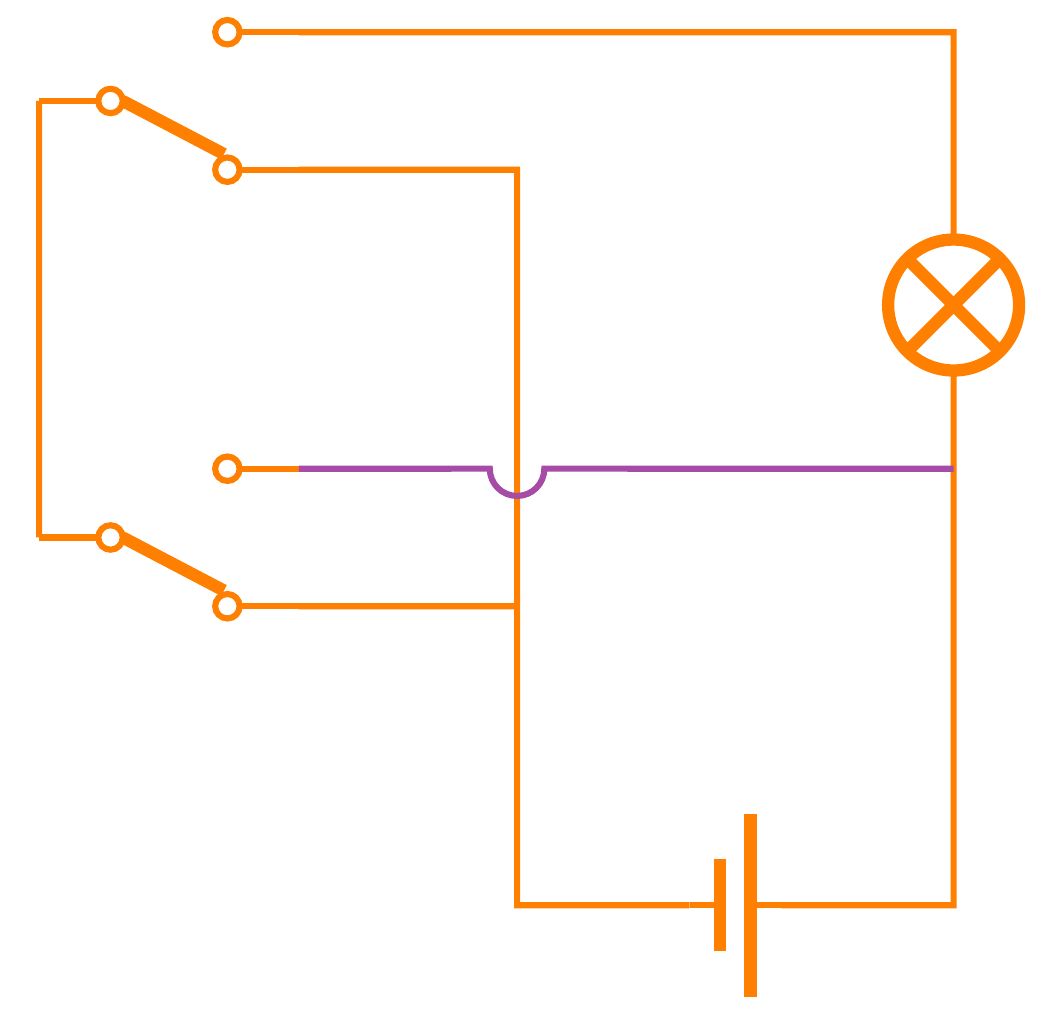
\includegraphics[width=0.50\textwidth]{gambar/Electric_circuit}}
	\caption{Contoh Penggambaran}
	\label{contoh}
\end{figure}	

\noindent
Berikut ini adalah gambar dari source code yang diatas.
\par 

\noindent 
Sementara Tikz menawarkan banyak fitur dan paket untuk membuat diagram dan segala macam gambar lainnya, namun sayangnya tidak ada paket yang bagus untuk tata letak sirkuit listrik. Dengan menggunakan paket circuitikz kita bisa dengan mudah menyelesaikan masalah ini. Ini meluas menyediakan lingkungan baru circuitikz di mana kita dapat dengan mudah menarik sirkuit kita dalam waktu singkat. Sintaksnya sama persis seperti yang ditunjukkan pada pelajaran sebelumnya, jadi kita bisa langsung memulai dengan contoh kode sederhana:
\par

\begin{verbatim}
\ documentclass {article}
\ usepackage {tikz}
\ usepackage {circuitikz}
\ begin {document}
\ begin {figure} [h!]
\ begin {center}
\ begin {circuitikz}
\ draw (0,0)

\end{verbatim}


\noindent 
 ke [V, v = $\$$ U$ \_ $q $\$$] (0,2)$\%$ Sumber tegangan
\par


\noindent 
 ke [pendek] (2,2)
\par


\noindent 
 ke [R = $\$$ R$ \_ $1 $\$$] (2,0)$\%$ Resistornya
\par


\noindent 
 ke [pendek] (0,0);
\par

\begin{verbatim}
\ end {circuitikz}
\ caption {sirkuit pertamaku.}
\ end {center}
\ end {figure}
\ end {document} 

\end{verbatim}

\noindent 
Sirkuit akan ditarik dengan cara yang sama seperti jalur di tikz, tapi kami menentukan opsi khusus untuk elemen:
\par


\noindent 
~ $\setminus$ draw (0,0)
\par


\noindent 
 ke [V, v = $\$$ U$ \_ $q $\$$] (0,2)$\%$ Sumber tegangan 
\par


\noindent 
Mulai dari (0,0) kita akan menggambar sumber tegangan yang menentukan opsi [V, v = UqUq] ke koordinat (0,2), di mana V memilih simbol untuk sumber tegangan dan v = UqUq Menarik panah voltase di sebelahnya. Lalu kita lanjutkan ke resistor:
\par


\noindent 
~ ke [pendek] (2,2)
\par


\noindent 
 ke [R = $\$$ R$ \_ $1 $\$$] (2,0)$\%$ Resistornya 
\par


\noindent 
Pertama kita harus menarik hubung singkat dari (0,2) ke (2,2) dan kemudian letakkan simbol resistor pada jalur dari (2,2) sampai (2,0) perhatikan bahwa kali ini label elemen harus ditentukan secara langsung ( R = R1R1 ) .
\par


\noindent 
Daftar semua elemen yang tersedia untuk rangkaian tersedia dalam manual circuitikz.
\par


\noindent 
Tapi bagaimana kita bisa menambahkan lebih banyak elemen ke sirkuit? Katakanlah kita ingin menambahkan sebuah induktor sejajar dengan Resistor. Cara termudah adalah dengan menambahkan perintah draw baru seperti ini:
\par


\noindent 
~ $\setminus$ begin $ \{ $circuitikz$ \} $
\par


\noindent 
 $\setminus$ draw (0,0)
\par


\noindent 
 ke [V, v = $\$$ U$ \_ $q $\$$] (0,2)$\%$ Sumber tegangan
\par


\noindent 
 ke [pendek] (2,2)
\par


\noindent 
 ke [R = $\$$ R$ \_ $1 $\$$] (2,0)$\%$ Resistornya
\par


\begin{enumerate}
	\item ke [pendek] (0,0);
	\item menarik (2,2)
	\item ke [pendek] (4,2)
	\item ke [L = $\$$ L$ \_ $1 $\$$] (4,0)
	\item ke [pendek] (2,0);
	\item end $ \{ $circuitikz$ \} $
\end{enumerate}



\noindent 
Menambahkan kapasitor di sampingnya, sama sederhananya:
\par


\noindent 
~ $\setminus$ begin $ \{ $circuitikz$ \} $
\par


\noindent 
 $\setminus$ draw (0,0)
\par


\noindent 
 ke [V, v = $\$$ U$ \_ $q $\$$] (0,2)$\%$ Sumber tegangan
\par


\noindent 
 ke [pendek] (2,2)
\par


\noindent 
 ke [R = $\$$ R$ \_ $1 $\$$] (2,0)$\%$ Resistornya
\par


\noindent 
 ke [pendek] (0,0);
\par


\noindent 
 menarik (2,2)
\par


\noindent 
 ke [pendek] (4,2)
\par


\noindent 
 ke [L = $\$$ L$ \_ $1 $\$$] (4,0)
\par


\noindent 
 ke [pendek] (2,0);
\par


\noindent 
 menarik (4,2)
\par


\noindent 
 ke [pendek] (6,2)
\par


\noindent 
 ke [C = $\$$ C$ \_ $1 $\$$] (6,0)
\par


\noindent 
 ke [pendek] (4,0);
\par


\noindent 
 $\setminus$ end $ \{ $circuitikz$ \} $ 
\par


\noindent 
Manual circuitikz memberikan contoh semua simbol dan fungsi dan juga dapat digunakan untuk referensi lebih lanjut.
\par

\subsection{Ringkasan}


\noindent 
Circuitikz menyediakan lingkungan untuk menggambar diagram sirkuit listrik
\par


\noindent 
Sintaksnya mirip dengan sintaks Tikz polos
\par


\noindent 
Daftar semua simbol tersedia dalam manual circutikz
\par


\noindent 
cara menggambar rangkaian listrik sederhana dalam dokumen LaTeX. Untuk melakukan ini kita akan menggunakan paket circuitikz yang berbasis pada paket TikZ. Untuk memulai kami mengisi paket circuitikz.
\par


\noindent 
$\setminus$usepackage$ \{ $circuitikz$ \} $ 
\par


\noindent 
Kami tidak perlu memuat paket TikZ juga karena secara otomatis dimuati dengan circuitikz.Untuk menggambar diagram kita menggunakan lingkungan circuitikz. Kami kemudian mengisi lingkungan dengan satu perintah $\setminus$draw berakhir dalam titik koma.
\par


\noindent 
 $\setminus$begin$ \{ $circuitikz$ \} $ $\setminus$draw <circuitikz code> ; $\setminus$end$ \{ $circuitikz$ \} $ 
\par


\noindent 
Format umum adalah sepasang koordinat yang diikuti oleh sebuah tautan dan kemudian pasangan koordinat berikutnya. Anda kemudian dapat terus menambahkan tautan dan koordinat lebih lanjut seperti rantai. Tautannya bisa berupa garis yang diraih dengan menggunakan dua tanda hubung, atau bisa juga komponen elektrik. Untuk menambahkan komponen pada sebuah garis kita menggunakan kata kunci 'to' diikuti dengan tanda kurung siku yang berisi nama komponen.
\par


\noindent 
Misalnya kita akan mulai dari (0,0) dan menuju ke (0,4) menambahkan baterai masuk. Kita kemudian akan menambahkan ammeter dalam perjalanan menuju (4,4) diikuti oleh garis sederhana ke (4 , 0). Kami akan menyelesaikan rangkaian dengan menambahkan lampu dalam perjalanan pulang (0,0).
\par


\noindent 
 $\setminus$begin$ \{ $circuitikz$ \} $ $\setminus$draw (0,0) to[battery] (0,4) to[ammeter] (4,4) -- (4,0) to[lamp] (0,0) ; $\setminus$end$ \{ $circuitikz$ \} $ 
\par


\noindent 
Inilah diagram yang terlihat seperti dikompilasi.
\par


\noindent 
Sekarang mari kita tambahkan voltmeter yang sejajar dengan lampu. Untuk melakukan ini, kami ingin bercabang dari garis bawah sepanjang jalan, lalu turun ke bawah, masukkan meter, lalu bergabung kembali dengan garis bawah sebelum akhirnya.
\par


\noindent 
 $\setminus$begin$ \{ $circuitikz$ \} $ $\setminus$draw (0,0) to[battery] (0,4) to[ammeter] (4,4) -- (4,0) to[lamp] (0,0) (0.5,0) -- (0.5,-2) to[voltmeter] (3.5,-2) -- (3.5,0) ; $\setminus$end$ \{ $circuitikz$ \} $ 
\par


\noindent 
Jika kita ingin membuat titik di mana garis bergabung ke terminal yang tepat yang diwakili oleh lingkaran, kita bisa menambahkan *-* ke dalam tanda kurung siku di mana kita menambahkan lampu masuk Ini akan menambahkan terminal di koordinat kedua sisi komponen . Oleh karena itu kita perlu memperpendek garis kedua sisi lampu sehingga terminal muncul di garis kita bergabung, dan kemudian kita perlu mengisi kekosongan.
\par


\noindent 
 $\setminus$begin$ \{ $circuitikz$ \} $ $\setminus$draw (0,0) to[battery] (0,4) to[ammeter] (4,4) -- (4,0) -- (3.5,0) to[lamp, *-*] (0.5,0) -- (0,0) (0.5,0) -- (0.5,-2) to[voltmeter] (3.5,-2) -- (3.5,0) ; $\setminus$end$ \{ $circuitikz$ \} $ 
\par


\noindent 
Selanjutnya kita akan menambahkan sebuah kapasitor di antara lampu dan ammeter. Kami tentukan kapasitor dengan modal C.
\par


\noindent 
 $\setminus$begin$ \{ $circuitikz$ \} $ $\setminus$draw (0,0) to[battery] (0,4) to[ammeter] (4,4) to[C] (4,0) -- (3.5,0) to[lamp, *-*] (0.5,0) -- (0,0) (0.5,0) -- (0.5,-2) to[voltmeter] (3.5,-2) -- (3.5,0) ; $\setminus$end$ \{ $circuitikz$ \} $ 
\par


\noindent 
Seringkali kami ingin menambahkan label ke diagram kami untuk memberi lebih banyak informasi kepada pembaca. Untuk dapat memasukkan unit listrik ke label kami, kami perlu menambahkan opsi 'siunitx' ke dalam $\setminus$usepackage .
\par


\noindent 
 $\setminus$usepackage[siunitx]$ \{ $circuitikz$ \} $ 
\par


\noindent 
Kita bisa menambahkan label ke ammeter seperti ini.
\par


\noindent 
 to[ammeter, l=2<$\setminus$ampere>] 
\par


\noindent 
'Saya mengatakan kepada LaTeX bahwa kami menambahkan sebuah label. Perhatikan bahwa kita menempatkan perintah unit dalam kurung kurawal. Karena kita menggunakan unit SI, kita bisa menambahkan awalan SI ke dalam. Kita juga bisa memindahkan label ke bawah simbol dengan menambahkan garis bawah segera setelah 'l'.
\par


\noindent 
 to[ammeter, l$ \_ $=2<$\setminus$milli$\setminus$ampere>] 
\par


\noindent 
Seperti yang kita tampilkan saat ini, kita bisa meletakkan label di sebelah panah di garis dengan mengubah 'l' menjadi 'i'.
\par


\noindent 
 to[ammeter, i$ \_ $=2<$\setminus$milli$\setminus$ampere>] 
\par


\noindent 
Mari tambahkan beberapa label di samping kapasitor dan voltmeter. Dengan kapasitor kita bisa saja memulai label dengan sama dengan mengikuti modal 'C'.
\par


\noindent 
 $\setminus$begin$ \{ $circuitikz$ \} $ $\setminus$draw (0,0) to[battery] (0,4) to[ammeter, i$ \_ $=2<$\setminus$milli$\setminus$ampere>] (4,4) to[C=3<$\setminus$farad>] (4,0) -- (3.5,0) to[lamp, *-*] (0.5,0) -- (0,0) (0.5,0) -- (0.5,-2) to[voltmeter, l=3<$\setminus$kilo$\setminus$volt>] (3.5,-2) -- (3.5,0) ; $\setminus$end$ \{ $circuitikz$ \} $ 
\par


\noindent 
Kita juga bisa mengubah warna komponen seperti ini.
\par


\noindent 
 to[voltmeter, l=3<$\setminus$kilo$\setminus$volt>, color=red] 
\par


\noindent 
Kita dapat mengubah ukuran diagram dengan menambahkan faktor penskalaan sebagai pilihan pada akhir perintah $\setminus$begin .
\par


\noindent 
 $\setminus$begin$ \{ $circuitikz$ \} $[scale=2] $\setminus$draw 
\par


\noindent 
Perhatikan bahwa komponen tetap berukuran sama namun jarak antar segala perubahan.
\par


\noindent 
Mari selesaikan postingan ini dengan melihat pilihan komponen lain yang bisa kita gunakan:
\par


\noindent 
 $\setminus$begin$ \{ $circuitikz$ \} $ $\setminus$draw (0,0) to[R, oo] (2,0) (4,0) to[vR, oo] (6,0) (0,2) to[transmission line, oo] (2,2) (4,2) to[closing switch, oo] (6,2) (0,4) to[european current source, oo] (2,4) (4,4) to[european voltage source, oo] (6,4) (0,6) to[empty diode, oo] (2,6) (4,6) to[full led, oo] (6,6) (0,8) to[generic, oo] (2,8) (4,8) to[sinusoidal voltage source, oo] (6,8) ; $\setminus$end$ \{ $circuitikz$ \} $ 
\par


\noindent 
Contoh ini semua bipoles.
\par


\noindent 
Dari kiri bawah kita miliki; sebuah resistor, resistor variabel, saluran transmisi, saklar penutup, sumber arus eropa, sumber tegangan eropa, dioda kosong, led penuh, bipol generik dan sumber tegangan sinusoidal.
\par


\noindent 
Bipoles bukan satu-satunya jenis komponen yang bisa kita gunakan. Kita juga bisa menambahkan monopoles, tripol, double bipoles, gerbang logika dan amplifier. Namun, kami tidak dapat menggunakan kata kunci 'to' untuk menambahkan ini seperti yang telah kami lakukan sebelumnya, karena keduanya tidak sesuai dengan satu baris saja. Sebagai gantinya kita menggunakan notasi node. Sebagai contoh, ini adalah bagaimana kita akan menampilkan antena:
\par


\noindent 
 (0,0) node[antenna] $ \{ $$ \} $ 
\par


\noindent 
Anda dapat menambahkan teks ke simbol menggunakan kurung kurawal, namun perhatikan bahwa kita masih perlu memasukkan kurung kurawal meskipun kita tidak ingin menggunakannya. Berikut adalah beberapa contoh lagi:
\par


\noindent 
 (4,0) node[pmos] $ \{ $$ \} $ (0,4) node[op amp] $ \{ $$ \} $ (4,4) node[american or port] $ \{ $$ \} $ (0,8) node[transformer] $ \{ $$ \} $ (4,8) node[spdt] $ \{ $$ \} $ 
\par


\noindent 
Untuk kemudian menghubungkannya dengan komponen lain, kita akan menggunakan jangkar simpul yang telah ditentukan. Untuk informasi lebih lanjut tentang semua komponen yang tersedia dan bagaimana Anda menghubungkan komponen menggunakan jangkar simpul, lihat dokumentasinya .
\par


\subsection{Pengantar}


\noindent 
Seperti yang kita pelajari di pelajaran 12, circuitikz adalah alat yang ampuh untuk pembuatan sirkuit. Tapi ada beberapa jebakan di sepanjang jalan. Manual circuitikz memberikan referensi bagus untuk semua komponen yang tersedia, namun tidak memiliki penjelasan mendalam tentang bagaimana menggunakan setiap elemen. Pada dasarnya, ada tiga jenis komponen penting yang tersedia di circuitikz, yaitu monopoles, bipoles dan tripole.Komponen lain yang disebutkan dalam manual dapat digunakan dengan cara yang mirip dengan kelas yang disebutkan dalam tutorial ini.
\par


\noindent 
Garis
\par


\noindent 
Sebelum saya masuk ke berbagai komponen, izinkan saya menunjukkan cara mengubah tampilan garis dasar di circuitikz.Perhatikan contoh berikut ini:
\par


\noindent 
~ $\setminus$ begin $ \{ $figure$ \} $ [h!]
\par


\noindent 
 $\setminus$ begin $ \{ $circuitikz$ \} $
\par


\noindent 
~~ $\setminus$ draw (-1,0) ke [pendek, oo] (1,0);
\par


\noindent 
 $\setminus$ end $ \{ $circuitikz$ \} $
\par


\noindent 
 $\setminus$ end $ \{ $figure$ \} $ 
\par


\noindent 
Seperti yang bisa Anda lihat, sintaksnya sedikit berubah dari pelajaran sebelumnya. Baris pertama hampir sama. Baris pertama akan menarik segmen garis atas dengan konektor terbuka di setiap ujungnya. Konektor dapat dipilih dengan mengubah bagian oo dalam kode.
\par


\noindent 
Jika kita ingin mengganti konektor, pertimbangkan contoh berikut, yang akan menghasilkan output ini:
\par


\noindent 
~ $\setminus$ begin $ \{ $figure$ \} $ [h!]
\par


\noindent 
 $\setminus$ begin $ \{ $circuitikz$ \} $
\par


\noindent 
~~ $\setminus$ draw (-1,0) ke [pendek, * -] (1,0);
\par


\noindent 
 $\setminus$ end $ \{ $circuitikz$ \} $
\par


\noindent 
 $\setminus$ end $ \{ $figure$ \} $ 
\par


\noindent 
Notasi untuk konektor cukup mudah. Anda bisa memilih jenis konektor di setiap ujung garis dengan menggunakan simbol * atau o. Selain itu Anda dapat memilih hanya satu ujung atau kedua ujung garis yang harus memiliki simbol semacam ini misalnya o-, -o atau oo. Jika Anda sama sekali tidak menginginkan konektor, cukup tulis ke [pendek] tanpa simbol tambahan.
\par


\noindent 
Monopoles
\par


\noindent 
Saya akan memulai dengan monopoles, yang merupakan komponen sirkuit yang paling dasar. Kelas ini berisi simbol seperti ground nodes dan antenna. Jadi mari kita lihat lebih dekat contoh yang sebenarnya.
\par


\noindent 
~ $\setminus$ begin $ \{ $figure$ \} $ [h!]
\par


\noindent 
 $\setminus$ begin $ \{ $circuitikz$ \} $
\par


\noindent 
~~ $\setminus$ draw (-1,0) ke [pendek, oo] (1,0);
\par


\noindent 
~~ $\setminus$ draw (0,0) ke [short] node [ground] $ \{ $$ \} $ (0, -1);
\par


\noindent 
 $\setminus$ end $ \{ $circuitikz$ \} $
\par


\noindent 
 $\setminus$ end $ \{ $figure$ \} $ 
\par


\noindent 
Saya mengambil garis dari bagian pertama, namun menambahkan simpul ke tanah. Seperti yang Anda lihat, garis berbeda dalam komponen tidak ditentukan sebagai bipole yang menggunakan operator, tapi sebagai simpul tipe tanah (simpul [ground]). Sangat penting, bahwa setiap simpul memiliki label di tikz. Label ini dapat dibiarkan kosong, namun sintaksnya harus berupa simpul [options] $ \{ $$ \} $. Jika kita memutuskan untuk memberi nama simpul kita, kita bisa menulis teks di antara kawat gigi seperti
\par


\noindent 
~ $\setminus$ begin $ \{ $figure$ \} $ [h!]
\par


\noindent 
 $\setminus$ begin $ \{ $circuitikz$ \} $
\par


\noindent 
~~ $\setminus$ draw (-1,0) ke [pendek, oo] (1,0);
\par


\noindent 
~~ $\setminus$ draw (0,0) ke [short] node [ground] $ \{ $GND$ \} $ (0, -1);
\par


\noindent 
 $\setminus$ end $ \{ $circuitikz$ \} $
\par


\noindent 
 $\setminus$ end $ \{ $figure$ \} $ 
\par


\noindent 
Itu semua ada pada monopoles di circuitikz.
\par


\noindent 
Bipoles
\par


\noindent 
Saya sudah membahas bipoles di pelajaran 12, tapi saya ingin menjelaskan beberapa fitur lanjutan lainnya di sini. Sebagian besar waktu, kita ingin memiliki panah untuk menunjukkan arus atau tegangan di sirkuit kita. Circuitikz menyediakan pilihan yang mudah digunakan untuk menambahkannya ke sirkuit Anda. Contoh di sini pada dasarnya diambil dari manual circuitikz, jadi Anda bisa menemukan beberapa contoh lagi di sana, tapi saya pikir mereka seharusnya tidak hilang dalam tutorial saya, karena ini adalah fitur yang sangat penting.
\par


\noindent 
Panah saat ini
\par


\noindent 
Cara paling dasar untuk menambahkan panah saat ini ke bipole Anda adalah dengan menentukan pilihan i untuk komponen masing-masing. Secara default, arah panah dan posisi label ditentukan oleh circuitikz, namun Anda dapat mengganti pengaturan tersebut untuk meningkatkan keterbacaan.
\par


\noindent 
~ $\setminus$ begin $ \{ $figure$ \} $ [h!]
\par


\noindent 
 $\setminus$ begin $ \{ $circuitikz$ \} $
\par


\noindent 
~~ $\setminus$ draw (0,0) ke [R, i = $\$$ i$ \_ $1 $\$$] (2,0);
\par


\noindent 
 $\setminus$ end $ \{ $circuitikz$ \} $
\par


\noindent 
 $\setminus$ end $ \{ $figure$ \} $ 
\par


\noindent 
Jika Anda ingin mengubah arah panah, Anda bisa menggunakan kode berikut sebagai gantinya. Operator <atau> dapat digunakan untuk menunjukkan arah panah.
\par


\noindent 
~ $\setminus$ begin $ \{ $figure$ \} $ [h!]
\par


\noindent 
 $\setminus$ begin $ \{ $circuitikz$ \} $
\par


\noindent 
~~ $\setminus$ draw (0,0) ke [R, i <= $\$$ i$ \_ $1 $\$$] (2,0);
\par


\noindent 
 $\setminus$ end $ \{ $circuitikz$ \} $
\par


\noindent 
 $\setminus$ end $ \{ $figure$ \} $ 
\par


\noindent 
Selanjutnya kita bisa memanipulasi posisi label i1i1 dengan menggunakan operator $ \string^ $ atau $ \_ $, yang berada di atas dan di bawah garis. Pertama lihat hasilnya untuk operator pertama:
\par


\noindent 
~ $\setminus$ begin $ \{ $figure$ \} $ [h!]
\par


\noindent 
 $\setminus$ begin $ \{ $circuitikz$ \} $
\par


\noindent 
~~ $\setminus$ draw (0,0) ke [R, i $ \string^ $ = $\$$ i$ \_ $1 $\$$] (2,0);
\par


\noindent 
 $\setminus$ end $ \{ $circuitikz$ \} $
\par


\noindent 
 $\setminus$ end $ \{ $figure$ \} $
\par


\noindent 
Sekarang kita ingin menempatkan label di bawah ini:
\par


\noindent 
~ $\setminus$ begin $ \{ $figure$ \} $ [h!]
\par


\noindent 
 $\setminus$ begin $ \{ $circuitikz$ \} $
\par


\noindent 
~~ $\setminus$ draw (0,0) ke [R, i $ \_ $ = $\$$ i$ \_ $1 $\$$] (2,0);
\par


\noindent 
 $\setminus$ end $ \{ $circuitikz$ \} $
\par


\noindent 
 $\setminus$ end $ \{ $figure$ \} $ 
\par


\noindent 
Dua jenis operator dapat dikombinasikan untuk mengubah posisi panah ke sisi kiri atau kanan bipole. Untuk menempatkan panah di sisi kiri, cukup tulis
\par


\noindent 
~ $\setminus$ begin $ \{ $figure$ \} $ [h!]
\par


\noindent 
 $\setminus$ begin $ \{ $circuitikz$ \} $
\par


\noindent 
~~ $\setminus$ draw (0,0) ke [R, i <$ \_ $ = $\$$ i$ \_ $1 $\$$] (2,0);
\par


\noindent 
 $\setminus$ end $ \{ $circuitikz$ \} $
\par


\noindent 
 $\setminus$ end $ \{ $figure$ \} $ 
\par


\noindent 
dan ubah arah untuk menempatkannya di sisi kanan seperti ini
\par


\noindent 
~ $\setminus$ begin $ \{ $figure$ \} $ [h!]
\par


\noindent 
 $\setminus$ begin $ \{ $circuitikz$ \} $
\par


\noindent 
~~ $\setminus$ draw (0,0) ke [R, i $ \_ $> = $\$$ i$ \_ $1 $\$$] (2,0);
\par


\noindent 
 $\setminus$ end $ \{ $circuitikz$ \} $
\par


\noindent 
 $\setminus$ end $ \{ $figure$ \} $ 
\par


\noindent 
Panah voltase
\par


\noindent 
Panah tegangan bisa digunakan dengan cara yang sama seperti panah saat ini, tapi kali ini, gunakan opsi v sebagai gantinya.
\par


\noindent 
~ $\setminus$ begin $ \{ $figure$ \} $ [h!]
\par


\noindent 
 $\setminus$ begin $ \{ $circuitikz$ \} $
\par


\noindent 
~~ $\setminus$ draw (0,0) ke [R, v $ \_ $> = $\$$ v$ \_ $1 $\$$] (2,0);
\par


\noindent 
 $\setminus$ end $ \{ $circuitikz$ \} $
\par


\noindent 
 $\setminus$ end $ \{ $figure$ \} $ 
\par


\noindent 
Seperti yang bisa Anda lihat, operator yang sama berlaku untuk memanipulasi posisi dan arah panah
\par


\noindent 
~ $\setminus$ begin $ \{ $figure$ \} $ [h!]
\par


\noindent 
 $\setminus$ begin $ \{ $circuitikz$ \} $
\par


\noindent 
~~ $\setminus$ draw (0,0) ke [R, v $ \string^ $ <= $\$$ v$ \_ $1 $\$$] (2,0);
\par


\noindent 
 $\setminus$ end $ \{ $circuitikz$ \} $
\par


\noindent 
 $\setminus$ end $ \{ $figure$ \} $ 
\par


\noindent 
Label
\par


\noindent 
Tentu saja mungkin untuk menambahkan label untuk elemen itu sendiri juga. Kami melakukannya dengan menggunakan opsi l kali ini.
\par


\noindent 
~ $\setminus$ begin $ \{ $figure$ \} $ [h!]
\par


\noindent 
 $\setminus$ begin $ \{ $circuitikz$ \} $
\par


\noindent 
~~ $\setminus$ draw (0,0) ke [R, l $ \string^ $ = $\$$ R$ \_ $1 $\$$] (2,0);
\par


\noindent 
 $\setminus$ end $ \{ $circuitikz$ \} $
\par


\noindent 
 $\setminus$ end $ \{ $figure$ \} $ 
\par


\noindent 
Sebaiknya kita menempatkan label di bawah elemen juga, sekali lagi menggunakan operator $ \_ $:
\par


\noindent 
~ $\setminus$ begin $ \{ $figure$ \} $ [h!]
\par


\noindent 
 $\setminus$ begin $ \{ $circuitikz$ \} $
\par


\noindent 
~~ $\setminus$ draw (0,0) ke [R, l $ \_ $ = $\$$ R$ \_ $1 $\$$] (2,0);
\par


\noindent 
 $\setminus$ end $ \{ $circuitikz$ \} $
\par


\noindent 
 $\setminus$ end $ \{ $figure$ \} $ 
\par


\noindent 
Tripoles
\par


\noindent 
Kelompok komponen yang terakhir namun tak kalah pentingnya adalah tripol. Kelompok tripoles yang paling penting tentu saja adalah semua jenis transistor. Anda bisa menemukan keseluruhan daftar contoh untuk transistor beserta yang ini di manual circuitikz, tapi saya jelaskan bagaimana penggunaannya berbeda dari bipoles.
\par


\noindent 
~ $\setminus$ begin $ \{ $figure$ \} $ [h!]
\par


\noindent 
 $\setminus$ begin $ \{ $circuitikz$ \} $
\par


\noindent 
~~ $\setminus$ draw (0,0) node [npn] (npn1) $ \{ $$ \} $
\par


\noindent 
~~ (npn1.base) node [anchor = east] $ \{ $B$ \} $
\par


\noindent 
~~ (npn1.collector) node [anchor = south] $ \{ $C$ \} $
\par


\noindent 
~~ (npn1.emitter) node [anchor = north] $ \{ $E$ \} $;
\par


\noindent 
 $\setminus$ end $ \{ $circuitikz$ \} $
\par


\noindent 
 $\setminus$ end $ \{ $figure$ \} $ 
\par


\noindent 
Tripol adalah simpul dalam circuitikz seperti monopoles, tapi Anda harus menempatkan beberapa jangkar ke masing-masing konektor tripol. Pertama, Anda menentukan nama untuk simpul dalam tanda kurung. Dalam hal ini saya telah memilih nama npn1. Nama ini akan digunakan untuk referensi ke transistor kita nanti. Setelah itu, ketiga jangkar tersebut harus di atur seperti yang terlihat di atas.
\par


\noindent 
Kita sekarang bisa merujuk ke node dan melampirkan beberapa elemen lain ke transistor.
\par


\noindent 
~ $\setminus$ begin $ \{ $figure$ \} $ [h!]
\par


\noindent 
 $\setminus$ begin $ \{ $circuitikz$ \} $
\par


\noindent 
~~ $\setminus$ draw (0,0) node [npn] (npn1) $ \{ $$ \} $
\par


\noindent 
~~ (npn1.base) node [anchor = east] $ \{ $B$ \} $
\par


\noindent 
~~ (npn1.collector) node [anchor = south, xshift = 0.5cm] $ \{ $C$ \} $
\par


\noindent 
~~ (npn1.emitter) node [anchor = north] $ \{ $E$ \} $;
\par


\noindent 
~~ $\setminus$ draw (npn1.collector) ke [R] ++ (0,2);
\par


\noindent 
 $\setminus$ end $ \{ $circuitikz$ \} $
\par


\noindent 
 $\setminus$ end $ \{ $figure$ \} $ 
\par


\noindent 
Perhatikan bahwa saya menambahkan opsi xshift ke nodus, untuk mencegah agar label tidak tumpang tindih dengan elemen baru.Saya harap Anda menikmati penjelasan saya dan yang Anda temukan dengan menggunakan circuitikz jauh lebih membingungkan dari sekarang.
\par


\noindent 
Ringkasan
\par


\noindent 
Ada tiga komponen utama komponen dalam sirkuitikz
\par


\noindent 
Semua kelas lainnya bisa digunakan dengan cara yang mirip dengan kelas utama tersebut
\par


\noindent 
Contoh penggunaan disediakan dalam manual circuitikz
\par
